\section{Fission Gas Behaviour}

In this section, the behaviour of the two main gases produced by fission events (Xenon and Krypton) is addressed, with particular focus on the impact of this phenomenon on some design parameters, such as the height of the plenum.

Both Xe and Kr are chemically inert gases, with a combined fission yield around 30\% (this value includes even other fast-decay fission products, which will result in Xe and Kr within few minutes).

Due to fission events, there will be a constant production rate of fission gas atoms, distributed in the fuel, giving rise to two main phenomena: Fuel Gaseous Swelling and Fission Gas Release.

\subsection{Fission Gas Release}

Due to essentially diffusion, part of the gas created in the fuel will be released in the plenum. Xe and Kr will \textquotedblleft pollute\textquotedblright\ the He initially contained in the plenum, decreasing its thermal conductivity and increasing the internal pressure of the pin (additional moles of gas are being introduced in a fixed volume).

All these phenomena are always ongoing under irradiation and affect the thermo-mechanical behaviour of the fuel pin in a highly non-linear way. It is crucial, then, to be able to correctly predict and control them.

The problem is tackled through the Rate Theory Equations, coupled with some Cluster Dynamics considerations. The physics of the phenomenon is described at the grain scale, which is taken as the domain for the problem. The equations to solve are essentially two:

The equation to estimate the total amount of gas that is produced, a simple ODE:
\begin{equation}
    \frac{dP}{dt} = y \cdot \dot{F} \quad \text{with} \quad 
    \begin{cases}
        P \left(\frac{\text{at}}{\text{m}^3}\right): \text{gas produced} \\
        y: \text{fission yield (combined)} \\
        \dot{F}: \text{fission rate}
    \end{cases}
\end{equation}

The equation for the intra-granular behaviour of gases, merging the gas remaining in solution and the gas held inside bubbles in a single term named $G_M$, indicating the gas retained by the fuel grain itself: 
\begin{equation}
    \frac{dG_M}{dt} = D_{\text{eff}} \cdot \nabla^2 G_M + y \cdot \dot{F} \quad \text{with} \quad 
    \begin{cases}
        G_M \left(\frac{\text{at}}{\text{m}^3}\right): \text{gas retained by grain} \\
        D_{\text{eff}}: \text{effective diffusivity (embeds all the phenomena)}
    \end{cases}
\end{equation}

\subsection{Main Assumptions, Data, and Hypotheses}

\begin{itemize}
    \item Domain size: grain size $d_g=10\,\mu \text{m}$.
    \item The reference model for diffusivity is the one by Matzke, 1980:
          \begin{equation}
              D_{\text{eff}} [\text{m}^2/\text{s}] = D_0 \cdot \exp\left(-\frac{Q}{T}\right)
          \end{equation}
          \begin{equation}
              \text{with } D_0 = 5 \cdot 10^{-8}\,\text{m}^2/\text{s}, \quad Q = -40262, \quad T\,[\text{K}]= \text{temperature}
          \end{equation}
    \item The reference temperature $T_{\text{ref}}$ considered is the simple average of the three main axial temperatures at the centre of the fuel (first \textquotedblleft slice\textquotedblright, midplane, last \textquotedblleft slice\textquotedblright). This is a conservative hypothesis, as diffusivity is enhanced by high temperatures and the temperatures at the inner radius are the highest.
    \item The fission yield considered is the combined Xe and Kr one: $y=30\%$.
    \item The fission rate is computed through the expression:
          \begin{equation}
              \dot{F} = \Sigma_f \cdot \phi_{\text{avg}}
          \end{equation}
          Where the global macroscopic fission cross section is obtained combining the microscopic cross sections for all the isotopes in the analysed fuel configuration (see reference for cross-section data), and the average neutron flux is computed assuming an axial profile equivalent to the one for linear power, through a \textquotedblleft peak-to-average\textquotedblright\ factor.
    \item Initial conditions: $P(0) = 0; G_M(0) = 0$.
    \item Boundary conditions for $G_M$ (Booth, 1957):
          \begin{itemize}
              \item \textquotedblleft Zero\textquotedblright\ boundary at surface (perfect sink): $G_M(a) = 0$
              \item Symmetry at the centre: $\frac{dG_M(0)}{dr} = 0$
          \end{itemize}
    \item The solution would generally look like:
          \begin{figure}[h!]
              \centering
              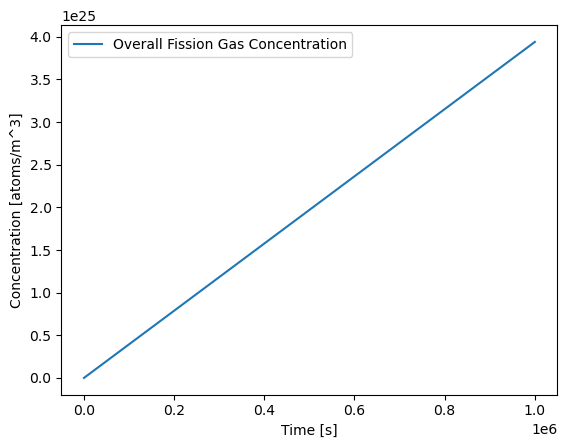
\includegraphics[width=0.8\textwidth]{FGR_1.png}
              \caption{Fission Gas Release dynamics and intra-granular behaviour of $G_M$.}
              \label{fig:FGR_1}
          \end{figure}
          \begin{figure}[h!]
              \centering
              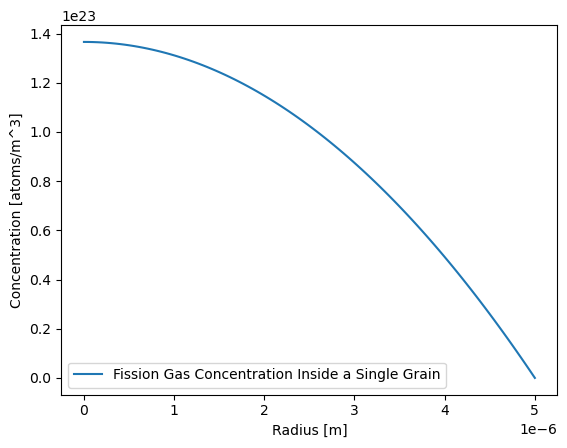
\includegraphics[width=0.8\textwidth]{FGR_2.png}
              \caption{Fission Gas Release over operational time.}
              \label{fig:FGR_2}
          \end{figure}
    \item The gas released is, then, the difference between the two shown quantities.
    \item As the timescale of the phenomenon is very small (fast) and the design must be targeted to one year of operation (360 effective days), the behaviour of the $G_M$ can be reasonably considered stabilized to the steady-state solution. \\
    The simplifying assumption made is then to neglect the time derivative in the equation, solving and integrating the simple remaining ODE on the specified domain.
    \item This model is considered suitable for describing the situation after the incubation time, which is neglected.
\end{itemize}

\subsection{Results and Comments}

\subsubsection{Total Gas Produced}

Here the actual solution for the fission gas production equation:
\begin{equation}
    \frac{dP}{dt} = Y_f \cdot \dot{F}
\end{equation}

\begin{figure}[h!]
    \centering
    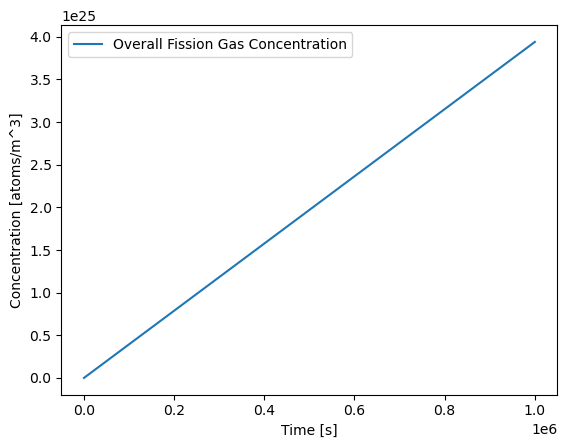
\includegraphics[width=0.8\textwidth]{FGR_1.png}
    \caption{Overall Fission Gas Concentration}
\end{figure}

By computing the value at $t = 360 \text{ days}$, the total gas produced is obtained.

\subsubsection{Gas Retained by Grain}

By solving the $G_M$ equation, the following spatial distribution is found:
\begin{figure}[h!]
    \centering
    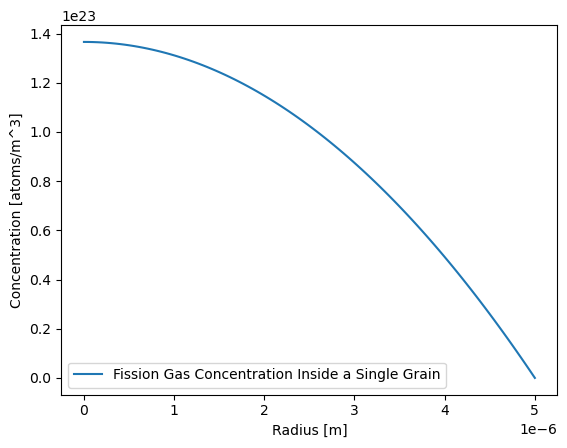
\includegraphics[width=0.8\textwidth]{FGR_2.png}
    \caption{Fission Gas Concentration Inside a Single Grain}
\end{figure}

Integrating this curve in the whole domain (grain size) and multiplying the obtained value for the number of grains in a fuel pellet (considered to be $10^5$) and the number of fuel pellets for each pin, the total amount of fission gas retained in the fuel is evaluated.

The total FGR is then the difference between the two quantities. Here the summary of the computed parameters and quantities:

\begin{table}[h!]
    \centering
    \caption{Summary of Computed Parameters and Quantities}
    \begin{tabular}{|c|c|}
        \hline
        \textbf{Parameter} & \textbf{Value} \\
        \hline
        $\Sigma_f$ & 0.027 cm$^{-1}$ \\
        $\phi_{\text{avg}}$ & $4.87 \cdot 10^{15}$ n/cm$^2 \cdot$ s \\
        $\dot{F}$ & $1.31 \cdot 10^{20}$ fissions/m$^3 \cdot$ s \\
        $T_{\text{avg}}$ & 2349.25 K \\
        $D_{\text{eff}}$ & $1.8 \cdot 10^{-15}$ m$^2$/s \\
        $P(1y)$ & $1.23 \cdot 10^{27}$ at/m$^3$ \\
        $G_M(1y)$ & $1.10 \cdot 10^{25}$ at/m$^3$ \\
        FGR & $1.21 \cdot 10^{27}$ at/m$^3$ \\
        \hline
    \end{tabular}
    \label{tab:fgr_summary}
\end{table}

\noindent \textbf{N.B.} Considering the orders of magnitude, a wise simplification would have been to directly neglect the gas retained in the grain and assume the totality of the gas produced as immediately released in the plenum. This hypothesis is also supported by the very high temperature characterizing the problem.

\subsection{Impact on the Design}

The FGR will increase the internal pressure of the fuel pin. Although it is not a major concern regarding the interaction with the coolant (which is almost at atmospheric pressure), it may be an issue for the stainless-steel cladding mechanical behaviour. Too high internal pressure would result in the cladding being too much under tension, affecting its mechanical properties.

To avoid very strong effects on the cladding, a limit on the internal pressure of the pin is set to $5 \, \text{MPa}$.

Considering the height of the plenum fixed, it is then possible to evaluate the new pressure of the filling gas (now "polluted") by a simple application of the ideal gas law:
\begin{equation}
    p \cdot V = n \cdot R \cdot T
\end{equation}
in which $n$ will increase (release of new gas) and the temperature is considered to be locked to the initial value for the filling gas (20°C).

By considering a set of possible plenum heights, the acceptable ones will be leading to new internal pressure below the just cited limit.

\begin{figure}[h!]
    \centering
    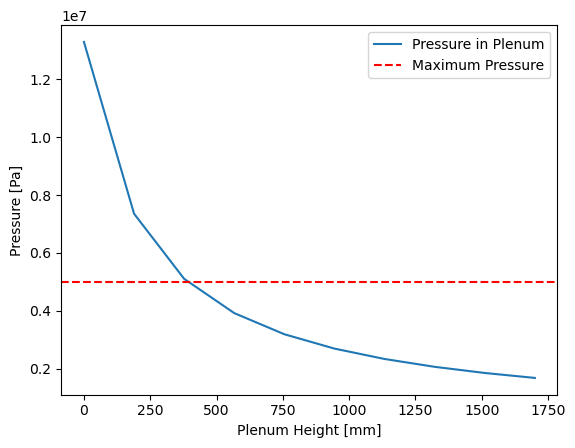
\includegraphics[width=0.9\textwidth]{FGR_3.png}
    \caption{Pressure in Plenum vs Plenum Height}
    \label{fig:plenum_pressure}
\end{figure}

As already mentioned, FGR will impact also on the thermal conductivity of the filling gas of the gap by reducing it. The conductivity worsening will lead to an increase in the fuel temperature. As diffusion processes are, in fact, temperature-driven, this will result in a higher Fission Gas Release.

The designer will then have to deal with a "positive feedback" phenomenon, eventually stopped and stabilized by thermal expansion effects.

For this reason, both phenomena are considered in sequence, with an iterative calculation logic, to reach convergence with some specific temperature and FGR values.
